\documentclass[letter,12pt]{article}
\usepackage[paperheight=27.94cm,paperwidth=21.59cm,bindingoffset=0in,left=3cm,right=2.0cm, top=3.5cm,bottom=2.5cm, headheight=15pt, headsep=1.0\baselineskip]{geometry}
\usepackage{graphicx,lastpage}
\graphicspath{{img/}}
\usepackage{upgreek}
\usepackage{censor}
\usepackage[spanish,es-tabla]{babel}
\usepackage{pdfpages}
\usepackage{tabularx}
\usepackage{graphicx}
\usepackage{adjustbox}
\usepackage[table]{xcolor}
\usepackage{colortbl}
\usepackage{rotating}
\usepackage{multirow}
\usepackage[utf8]{inputenc}
\usepackage{float}
\usepackage{hyperref}
\usepackage{tikz}
\usetikzlibrary{positioning, arrows.meta, fit}

\renewcommand{\tablename}{Tabla}
\usepackage{fancyhdr}
\pagestyle{fancy}
\fancyhf{}
\fancyfoot[C]{\thepage}
\renewcommand{\headrulewidth}{0.4pt}
\makeatletter
\newcommand{\hdrmark}{%
  \protected@edef\@tempa{\rightmark}%
  \ifx\@tempa\@empty\nouppercase{\leftmark}\else\nouppercase{\rightmark}\fi}
\makeatother
\fancyhead[L]{\hdrmark}


%
\begin{document}
%
   \title{\Huge{Informe Laboratorio 2}}

   \author{\textbf{Sección 1} \\  \\Alumno Maximiliano Solorza \\ e-mail: maximiliano.solorza@mail.udp.cl}

   \date{Septiembre de 2026}

   \maketitle

   \tableofcontents

  \newpage


\section{Descripción de actividades}
Utilizando la aplicación web vulnerable DVWA

(Damn Vulnerable Web App - \href{https://github.com/digininja/DVWA}{https://github.com/digininja/DVWA} (Enlaces a un sitio externo.)) realice las siguientes actividades:


\begin{itemize}
    \item Despliegue la aplicación en su equipo utilizando docker. Detalle el procedimiento y explique los parámetros que utilizó.
    \item Utilice Burpsuite (https://portswigger.net/burp/communitydownload (Enlaces a un sitio externo.)) para realizar un ataque de fuerza bruta contra formulario ubicado en vulnerabilities/brute. Explique el proceso y obtenga al menos 2 pares de usuario/contraseña válidos. Muestre las diferencias observadas en burpsuite.
    \item Utilice la herramienta cURL, a partir del código obtenido de inspect elements de su navegador, para realizar un acceso válido y uno inválido al formulario ubicado en vulnerabilities/brute. Indique 4 diferencias entre la página que retorna el acceso válido y la página que retorna un acceso inválido.
    \item Utilice la herramienta Hydra para realizar un ataque de fuerza bruta contra formulario ubicado en vulnerabilities/brute. Explique el proceso y obtenga al menos 2 pares de usuario/contraseña válidos.
    \item Compare los paquetes generados por hydra, burpsuite y cURL. ¿Qué diferencias encontró? ¿Hay forma de detectar a qué herramienta corresponde cada paquete?
\end{itemize}

\newpage

\section{Desarrollo de actividades según criterio de rúbrica}

\subsection{Levantamiento de docker para correr DVWA (dvwa)}
El entorno de trabajo es \textbf{Kali Linux sobre WSL2} (WSL v2.6.2) en Windows~11. Dado que DVWA es,
por diseño, una aplicación \emph{deliberadamente vulnerable}, el despliegue se planteó de modo que el
servicio no resulte alcanzable desde fuera del propio equipo: se publica únicamente en
\texttt{127.0.0.1}, la base de datos no expone puerto alguno y ambos contenedores corren sin
privilegios adicionales. De forma independiente, y como simple medida preventiva frente a errores propios (un \texttt{rm} mal tipeado, un comodín de más en un script), se deshabilitó el
\texttt{automount} de \texttt{/mnt/c} en \texttt{/etc/wsl.conf}, de modo que el disco \texttt{C:} de
Windows no queda montado dentro de Kali.
\\

Como paso previo se instaló el \emph{Docker Engine} nativo dentro de Kali (no Docker Desktop, que se
integra con Windows), gestionado por systemd:

\begin{figure}[H]
    \centering
    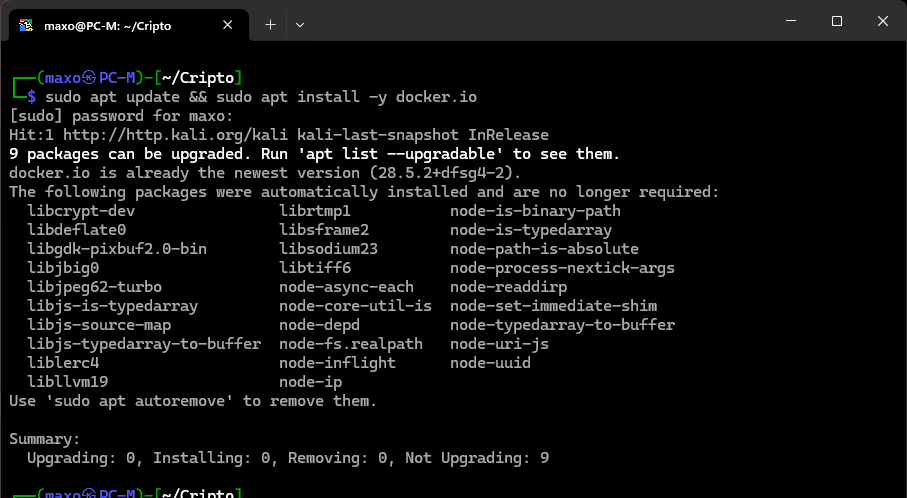
\includegraphics[width=0.9\textwidth]{instalardocker.png}
    \caption{Instalación de Docker Engine (paquete \texttt{docker.io}) en Kali.}
\end{figure}

\begin{figure}[H]
    \centering
    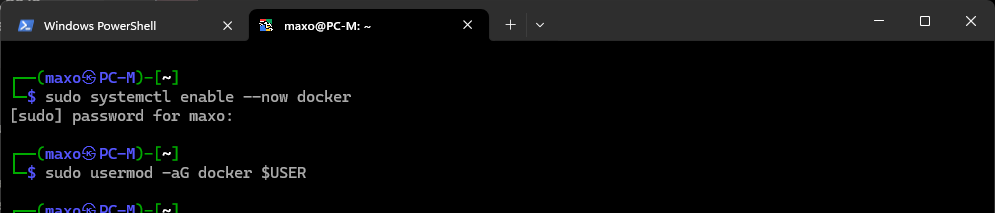
\includegraphics[width=0.9\textwidth]{activardocker.png}
    \caption{Habilitación e inicio del servicio Docker mediante systemd.}
\end{figure}

\begin{figure}[H]
    \centering
    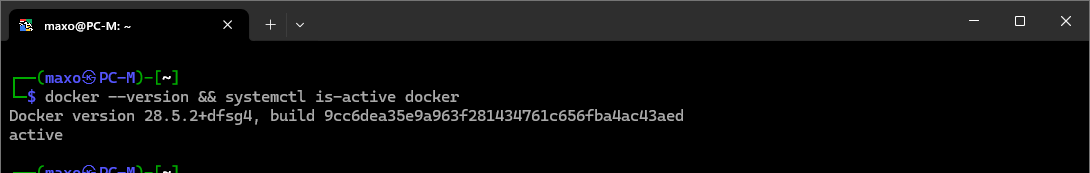
\includegraphics[width=0.9\textwidth]{verificarversionygruo.png}
    \caption{Verificación: Docker 28.5.2 instalado y servicio en estado \texttt{active}.}
\end{figure}

Ya con el motor disponible, se utilizó la imagen oficial mantenida por el autor del proyecto
(\texttt{ghcr.io/digininja/dvwa}), acompañada de un contenedor de base de datos \texttt{mariadb:lts}.
El procedimiento de despliegue fue el siguiente:

\begin{enumerate}
    \item Descargar la imagen oficial \texttt{ghcr.io/digininja/dvwa:latest} desde el registro público.
    \item Crear una red \emph{bridge} dedicada (\texttt{dvwa-net}) y levantar sobre ella los dos contenedores: la base de datos \texttt{mariadb:lts} \textbf{sin publicar puerto} (solo alcanzable dentro de esa red) y DVWA \textbf{publicada únicamente en \texttt{127.0.0.1:4280}}, ambos sin privilegios adicionales (\texttt{no-new-privileges}) y con límites de CPU y memoria. El comando completo y su ejecución se muestran en la Figura~\ref{fig:levantar}.
    \item Acceder a la aplicación desde el navegador en \texttt{http://localhost:4280/}.
    \item Iniciar sesión con las credenciales por defecto \texttt{admin / password}.
    \item Presionar el botón \textbf{Create / Reset Database} para inicializar la base de datos MySQL/MariaDB (siembra los 5 usuarios por defecto).
    \item En \textbf{DVWA Security} configurar el nivel de seguridad en \textbf{Low}, requisito para que el formulario de \texttt{vulnerabilities/brute} sea vulnerable a fuerza bruta.
\end{enumerate}

%\textbf{Explicación de los parámetros utilizados:}
%\begin{itemize}
 %   \item \texttt{docker run}: crea y ejecuta un nuevo contenedor a partir de una imagen.
 %  \item \texttt{-d} (detached): ejecuta el contenedor en segundo plano.
  %  \item \texttt{-{}-name}: asigna un nombre fijo al contenedor (\texttt{dvwa}, \texttt{dvwa-db}) para gestionarlo con facilidad.
   % \item \texttt{-{}-network dvwa-net}: conecta el contenedor a una red \emph{bridge} dedicada y aislada.
    %\item \texttt{-p 127.0.0.1:4280:80}: publica el puerto (redirección) en formato \texttt{IP\_host:puerto\_host:puerto\_contenedor}; al fijar \texttt{127.0.0.1} el servicio solo queda accesible desde \emph{localhost}.
    %\item \texttt{-{}-security-opt no-new-privileges}: impide que los procesos del contenedor escalen privilegios.
    %\item \texttt{-{}-restart unless-stopped}: reinicia el contenedor automáticamente salvo que se detenga manualmente.
    %\item \texttt{-{}-cpus} / \texttt{-{}-memory}: limitan los recursos que el contenedor puede consumir.
    %item \texttt{-e VARIABLE=valor}: define variables de entorno (aquí, los datos de conexión a la base de datos).
    %\item \texttt{ghcr.io/digininja/dvwa:latest} / \texttt{mariadb:lts}: nombres de las imágenes que se ejecutan.
%\end{itemize}

\begin{figure}[H]
    \centering
    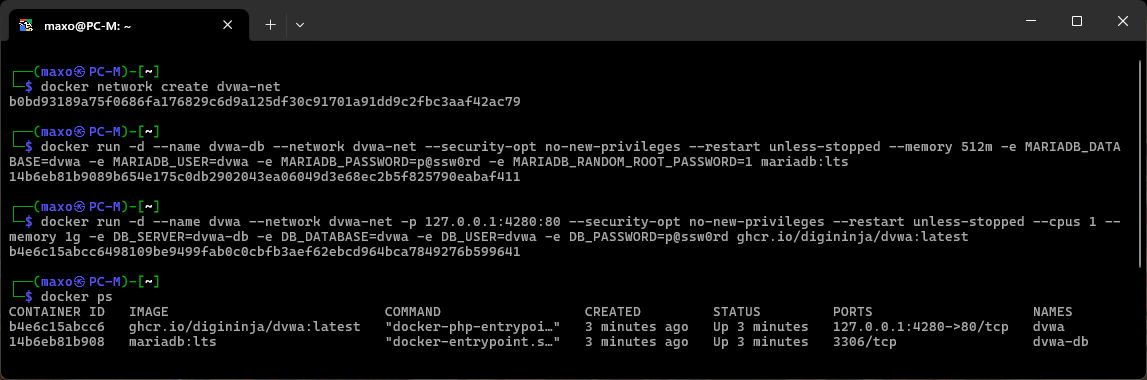
\includegraphics[width=0.9\textwidth]{levantardocker.png}
    \caption{Creación de la red dedicada y levantamiento de los contenedores DVWA y MariaDB.}
    \label{fig:levantar}
\end{figure}

\begin{figure}[H]
    \centering
    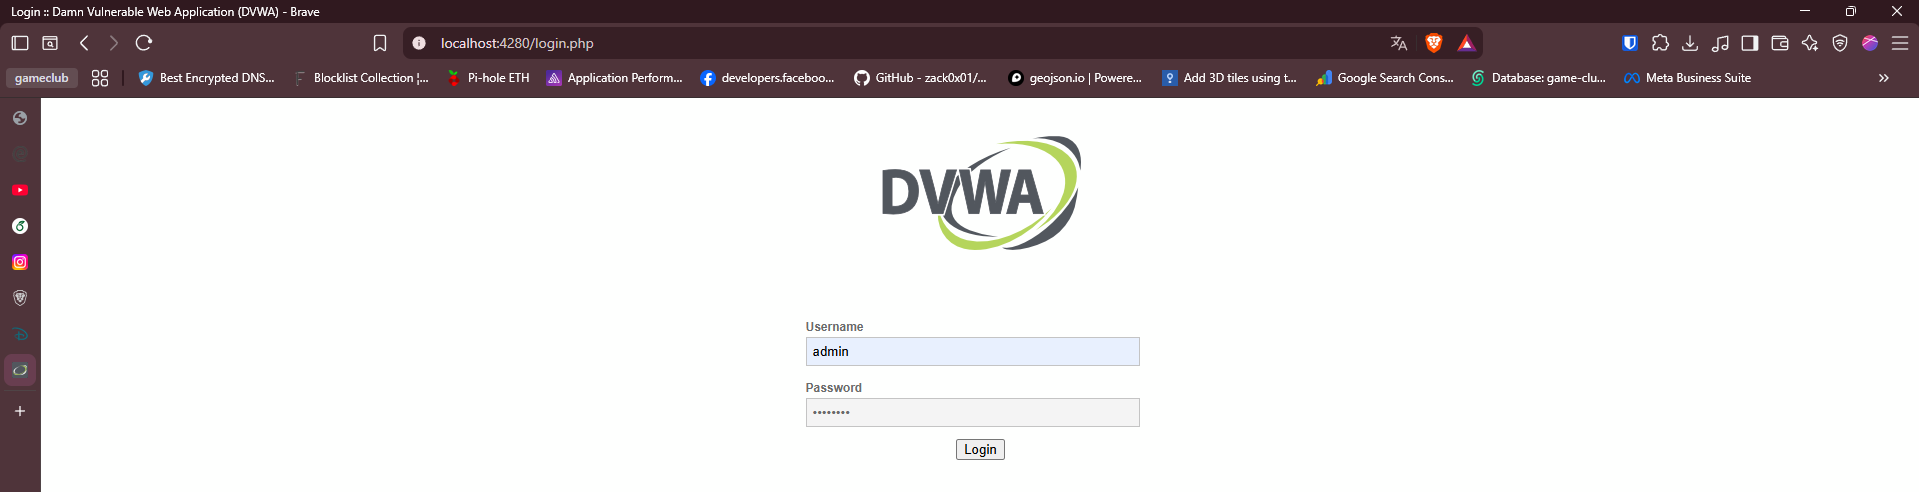
\includegraphics[width=0.9\textwidth]{loginlocal.png}
    \caption{Acceso a DVWA en \texttt{http://localhost:4280} con las credenciales por defecto \texttt{admin/password}.}
\end{figure}

\begin{figure}[H]
    \centering
    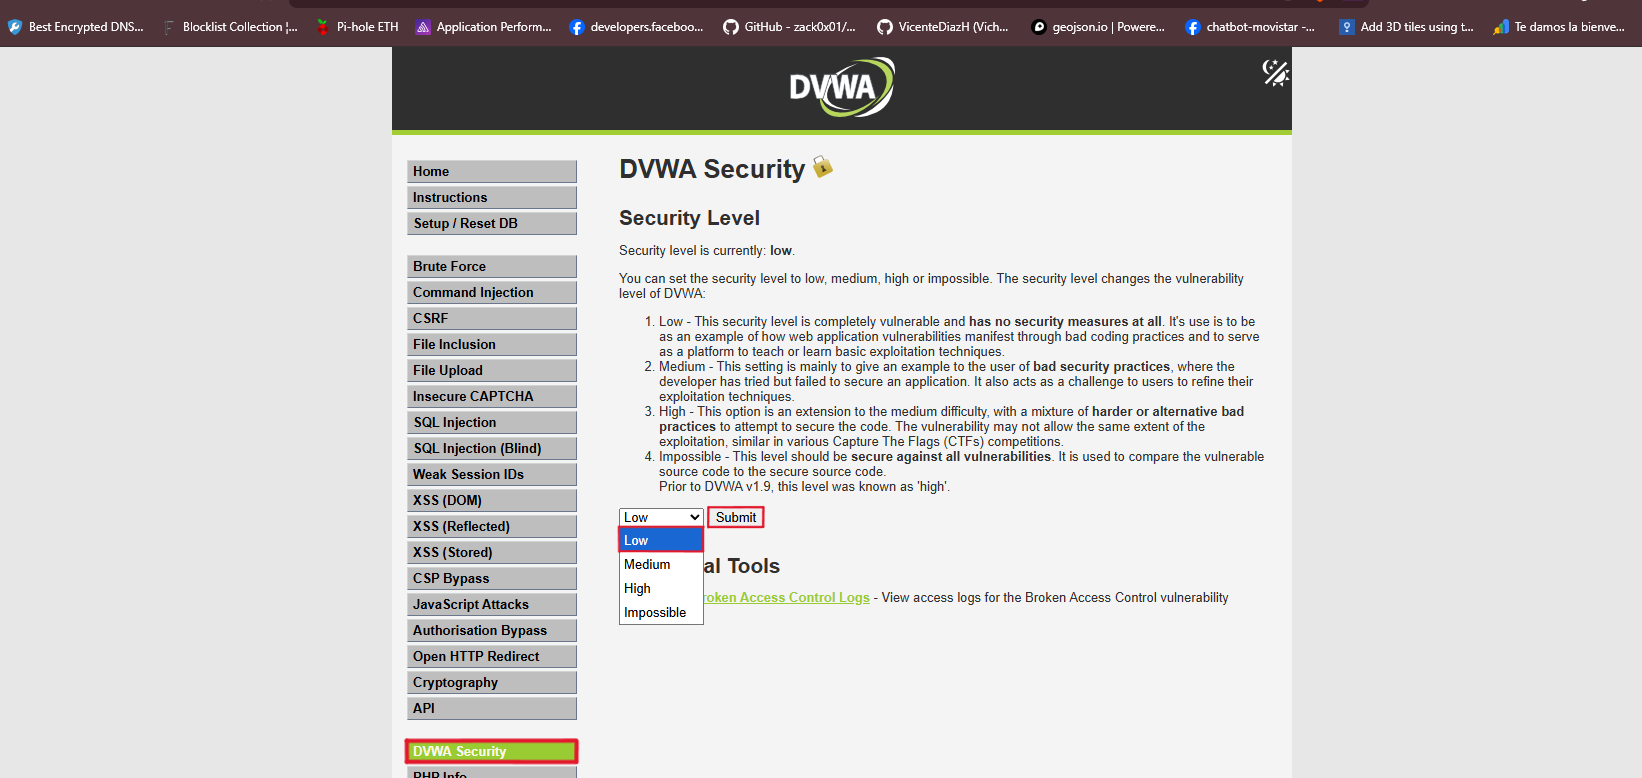
\includegraphics[width=0.9\textwidth]{nivelseguridadLOW.png}
    \caption{Configuración del nivel de seguridad de DVWA en \textbf{Low}.}
    \label{fig:low}
\end{figure}

Tal como lo solicita el enunciado, el nivel de seguridad de DVWA se configuró en \textbf{Low} (Figura~\ref{fig:low}). Este es el nivel requerido para que el formulario de \texttt{vulnerabilities/brute} sea susceptible al ataque de fuerza bruta, ya que en los niveles superiores (\emph{Medium} y \emph{High}) DVWA incorpora protecciones adicionales.
\\


\subsection{Redirección de puertos en docker (dvwa)}
La redirección de puertos se controla con el flag \texttt{-p [IP\_host:]puerto\_host:puerto\_contenedor}. DVWA corre Apache escuchando internamente en el puerto \textbf{80} del contenedor; con \texttt{-p 127.0.0.1:4280:80} ese puerto interno se expone en el puerto \textbf{4280} de la máquina anfitriona, pero \textbf{únicamente en la interfaz de loopback} (\texttt{127.0.0.1}), permitiendo el acceso vía \texttt{http://localhost:4280/} y evitando que el servicio quede expuesto a la red local. \\


Este detalle es clave desde el punto de vista de seguridad: si se hubiese usado \texttt{-p 4280:80} (o \texttt{-p 80:80}), Docker enlazaría el puerto en \texttt{0.0.0.0}, es decir en \emph{todas} las interfaces, y DVWA sería alcanzable desde cualquier equipo de la LAN, lo cual es inaceptable para una aplicación deliberadamente vulnerable. \\


Si el puerto elegido estuviera ocupado, basta con cambiar el puerto del host manteniendo el enlace a loopback, por ejemplo \texttt{-p 127.0.0.1:8080:80}, quedando disponible en \texttt{http://localhost:8080/}; internamente el contenedor sigue usando el puerto 80. \\


La redirección activa puede verificarse con \texttt{docker ps}, que en la columna \texttt{PORTS} muestra el mapeo, en este caso: \texttt{127.0.0.1:4280->80/tcp} (nótese el enlace a loopback y no a \texttt{0.0.0.0}). \\


Para dejar constancia de que la redirección quedó efectivamente restringida a \emph{loopback}, se comprobó el enlace desde ambos lados (Kali y Windows), como se muestra en la Figura~\ref{fig:aislamiento}: dentro de Kali el socket solo escucha en \texttt{127.0.0.1:4280} (\texttt{ss}) y DVWA responde por \emph{loopback} (\texttt{curl}, HTTP 302), mientras que un intento contra la IP de red de Kali es rechazado; del lado de Windows, \texttt{netstat} confirma el enlace a \texttt{127.0.0.1} y no a \texttt{0.0.0.0}. \\


\begin{figure}[H]
    \centering
    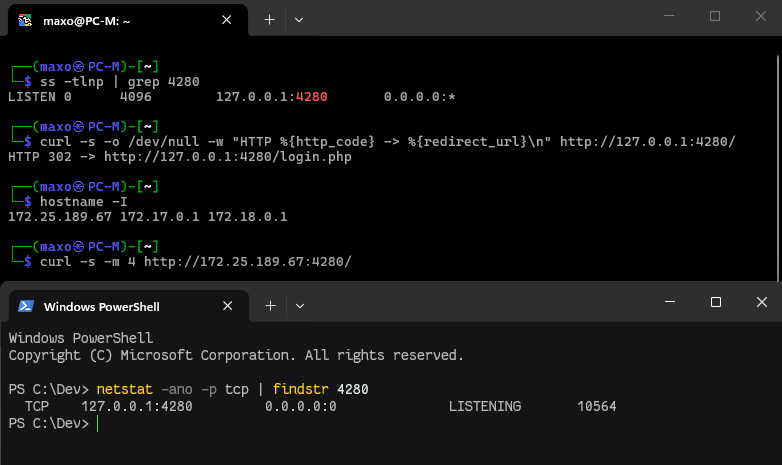
\includegraphics[width=0.9\textwidth]{verificacionaislamientored.png}
    \caption{Verificación del aislamiento de red: el servicio solo escucha en \emph{loopback} (\texttt{ss} en Kali, \texttt{netstat} en Windows), responde por \texttt{127.0.0.1} y resulta inalcanzable desde la IP de red de Kali.}
    \label{fig:aislamiento}
\end{figure}

El resultado confirma la postura buscada: DVWA es accesible únicamente desde el \texttt{localhost} de
Kali y desde el \texttt{localhost} de Windows (vía el reenvío de \emph{localhost} propio de WSL2), pero
\textbf{invisible para cualquier otra máquina de la red}. Cabe precisar que esta comprobación no cubre
al navegador del propio operador, para el cual \texttt{localhost} es una dirección alcanzable como
cualquier otra; de ahí que convenga detener los contenedores (\texttt{docker stop dvwa dvwa-db}) al
cerrar cada sesión de trabajo. \\


\subsection{Obtención de consulta a replicar (burp)}
Burp Suite Community se ejecutó dentro de Kali. Se utilizó su navegador embebido (\textbf{Proxy $\rightarrow$ Open browser}), que ya viene configurado para pasar el tráfico por el proxy de Burp en \texttt{127.0.0.1:8080}. \\


\begin{figure}[H]
    \centering
    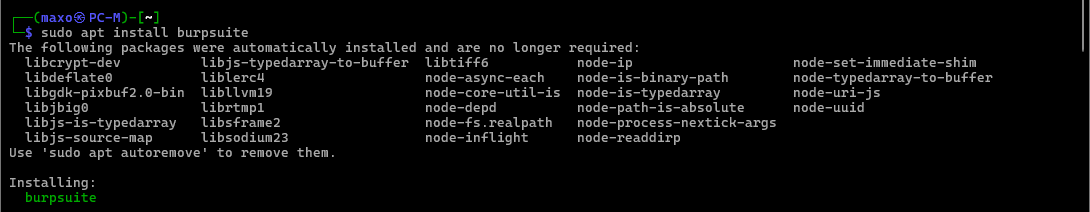
\includegraphics[width=0.7\textwidth]{instalarburpsuit.png}
    \caption{Instalación/inicio de Burp Suite Community en Kali.}
\end{figure}

El formulario objetivo es \texttt{Vulnerabilities $\rightarrow$ Brute Force} de DVWA:

\begin{figure}[H]
    \centering
    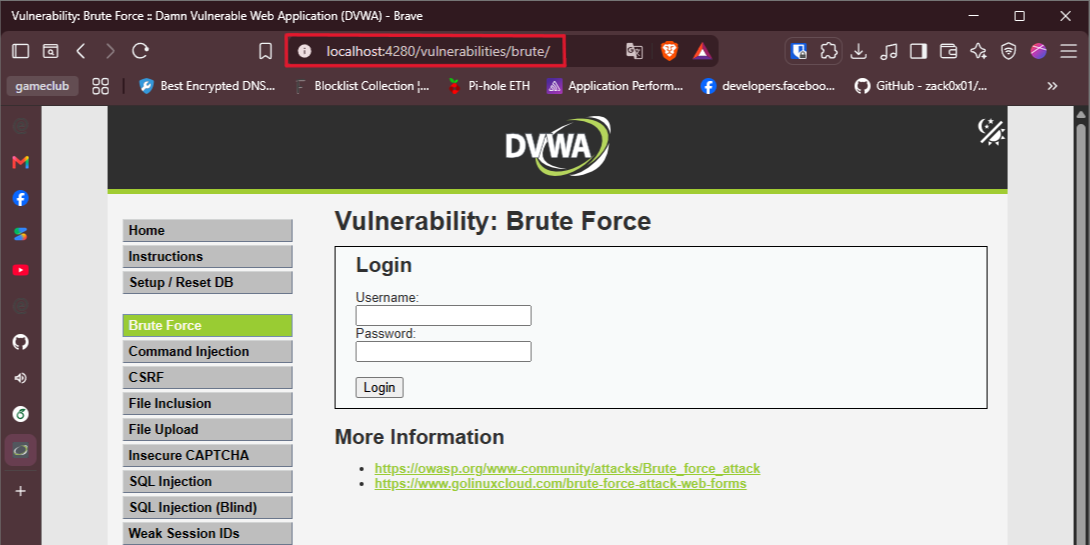
\includegraphics[width=0.9\textwidth]{bruteforce.png}
    \caption{Formulario objetivo: módulo \textit{Brute Force} de DVWA.}
\end{figure}

Con la opción \textbf{Intercept ON} en la pestaña \textit{Proxy}, se envió una solicitud de prueba desde el formulario ingresando un usuario y contraseña cualquiera. Burp capturó la petición HTTP. Como el nivel de seguridad es \textbf{Low}, el formulario envía los datos por método \textbf{GET}, por lo que \textbf{el usuario y la contraseña viajan visibles en la propia URL}\\

Se observan tres parámetros relevantes: \\

\texttt{username: prueba1} \\

\texttt{password: canyouseethis\_lilpadawan} \\

\texttt{PHPSESSID: 362db30f14d3ce1de1b596310a44196d} \\

\textbf{Es fundamental que la petición incluya la cookie \texttt{PHPSESSID} de una sesión ya autenticada}: sin ella, DVWA redirige cada solicitud a \texttt{login.php} (HTTP 302) y el ataque no llega al formulario (ver subsección de resultados). Esta petición interceptada se envió al módulo \textbf{Intruder} con clic derecho $\rightarrow$ \textit{Send to Intruder}. \\


\begin{figure}[H]
    \centering
    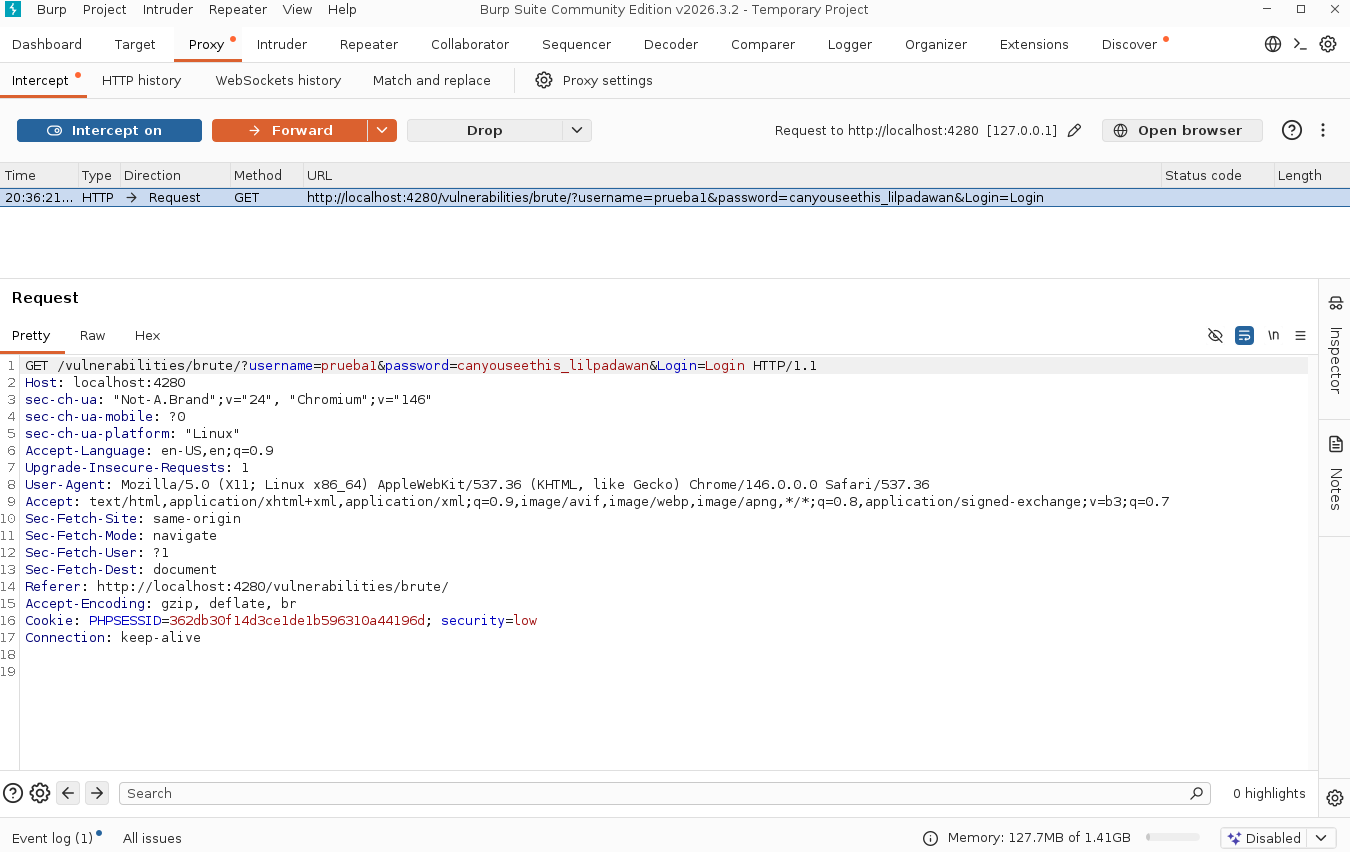
\includegraphics[width=0.95\textwidth]{primerburpsuitloginyclavervisibleenellink.png}
    \caption{Petición interceptada en Burp (Intercept ON): por el método GET, el usuario y la contraseña quedan expuestos en la URL.}
\end{figure}

\subsection{Identificación de campos a modificar (burp)}
Dentro del módulo \textbf{Intruder}, en la pestaña \textit{Positions}, Burp marca automáticamente los parámetros con el símbolo \texttt{\S}. Se limpiaron todas las marcas con \textbf{Clear \S} y luego se marcaron manualmente únicamente los campos \texttt{username} y \texttt{password} como posiciones de payload: \\


Al tener dos posiciones a probar de forma combinada, se seleccionó el tipo de ataque \textbf{Cluster bomb}, que prueba todas las combinaciones posibles de la lista de usuarios contra la lista de contraseñas. \\


\begin{figure}[H]
    \centering
    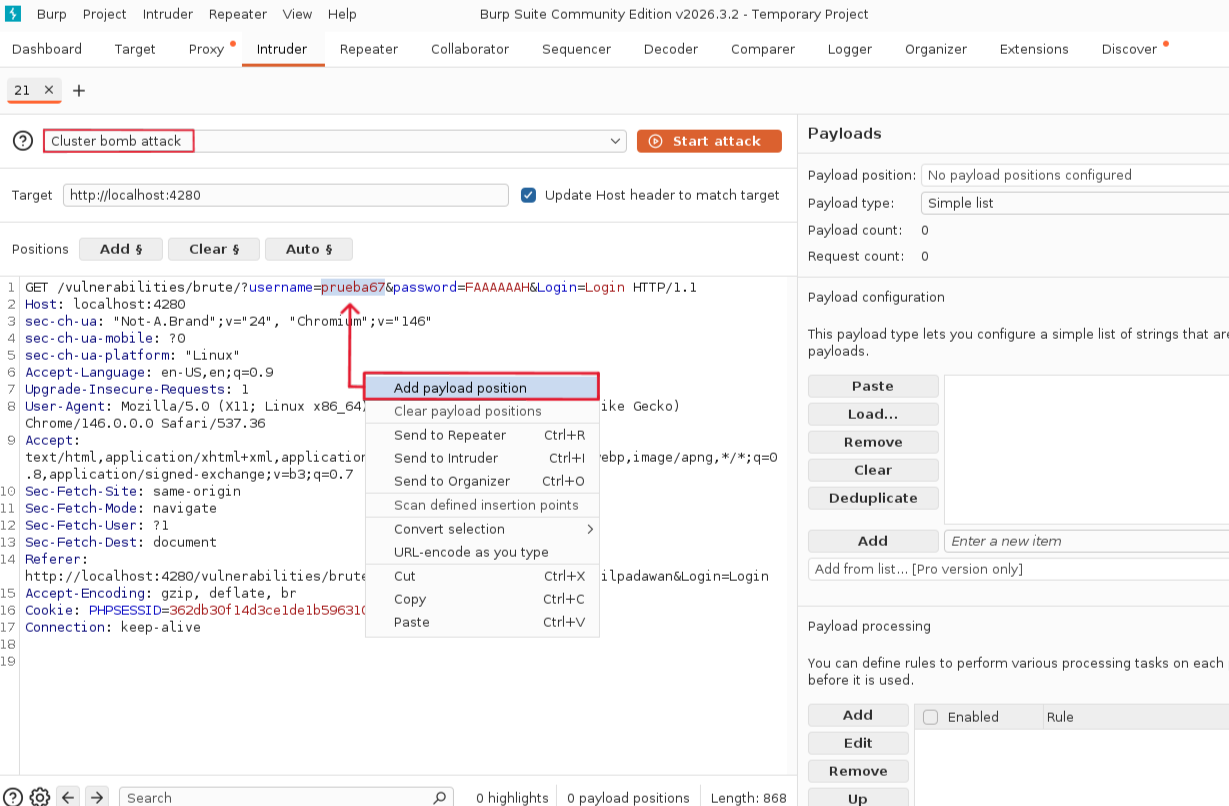
\includegraphics[width=0.95\textwidth]{addpayload.png}
    \caption{Marcado de las posiciones de payload (\texttt{username} y \texttt{password}) y selección del ataque \textbf{Cluster bomb} en Intruder.}
\end{figure}

\subsection{Obtención de diccionarios para el ataque (burp)}
\textbf{Contratiempo de memoria y \emph{throttling}.} Inicialmente se intentó usar el diccionario \texttt{rockyou.txt} (el volcado real de la brecha de RockYou de 2009, incluido en Kali en \texttt{/usr/share/wordlists/rockyou.txt.gz}, con más de 14 millones de contraseñas). Sin embargo, Burp Intruder \textbf{carga la lista completa en memoria}, por lo que el consumo de RAM se dispara y la herramienta se vuelve inutilizable. A esto se suma que la edición Community \textbf{limita deliberadamente la velocidad} de Intruder. Por ambos motivos se optó por un \textbf{diccionario reducido y dirigido}, obtenido enumerando el propio objetivo. \\


\textbf{Enumeración de usuarios (SQL Injection).} Los nombres de usuario propios de DVWA (\texttt{gordonb}, \texttt{1337}, \texttt{pablo}, \texttt{smithy}) no aparecen en ninguna wordlist genérica, por ser cuentas propias de la aplicación. Se obtuvieron mediante \textbf{SQL Injection} sobre \texttt{vulnerabilities/sqli} (nivel Low), aprovechando la consulta vulnerable \texttt{SELECT first\_name, last\_name FROM users WHERE user\_id='\$id'}. Con una inyección \texttt{UNION} se volcó la tabla \texttt{users} completa (usuario y hash): \\

\begin{verbatim}
1' UNION SELECT user, password FROM users #
\end{verbatim}
El \emph{username} aparece en la columna ``First name'' y el hash MD5 en ``Surname'', tal como se observa en la Figura~\ref{fig:sqli}.

\begin{figure}[H]
    \centering
    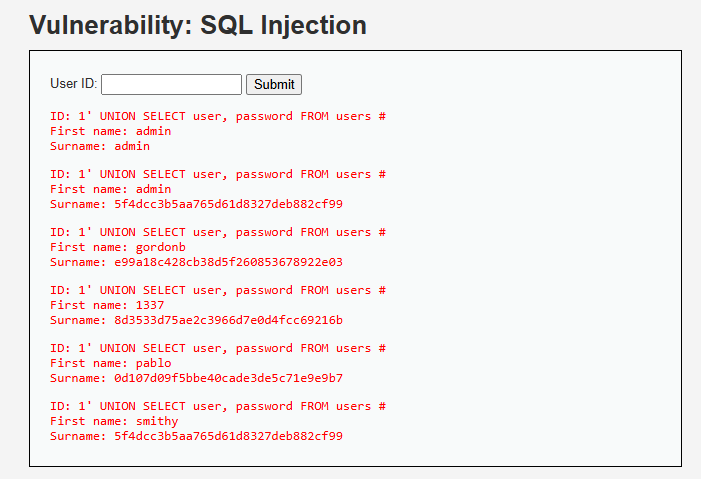
\includegraphics[width=0.95\textwidth]{SQLparatenerusers.png}
    \caption{Volcado de la tabla \texttt{users} (usuarios y hashes MD5) mediante SQL Injection.}
    \label{fig:sqli}
\end{figure}


\textbf{Diccionarios finales cargados en Intruder.} Con lo anterior se construyeron dos listas mínimas: un \texttt{users.txt} con los usuarios enumerados (más algunos genéricos: \texttt{root}, \texttt{user}, \texttt{guest}, \texttt{dragon}, \texttt{pepe})  y un \texttt{pass.txt} con una cabecera de contraseñas comunes de \texttt{SecLists}. Ambas listas caben holgadamente en memoria y evitan el \emph{throttling} excesivo, a diferencia de \texttt{rockyou} completo. \\


\subsection{Obtención de al menos 2 pares (burp)}
Con los diccionarios cargados y el ataque \textbf{Cluster bomb}, se lanzó Intruder. El formulario en nivel Low devuelve \textbf{siempre HTTP 200}: no cambia el código de estado, sino el \textbf{contenido} de la respuesta. Por eso el discriminador entre acierto y fallo es la \textbf{longitud de la respuesta (Length)}: \\


\begin{itemize}
    \item \textbf{Login inválido:} la página incluye \emph{``Username and/or password incorrect.''} $\rightarrow$ longitud \emph{baseline} constante.
    \item \textbf{Login válido:} la página incluye \emph{``Welcome to the password protected area''} y la imagen de avatar del usuario $\rightarrow$ su \textbf{Length difiere} de la baseline.
\end{itemize}

Ordenando los resultados por la columna \texttt{Length}, las filas con longitud distinta corresponden a las credenciales válidas. Se obtuvieron las siguientes credenciales: \\


\begin{table}[H]
\centering
\begin{tabular}{lll}
\hline
\textbf{Usuario} & \textbf{Contraseña} & \textbf{Length} \\
\hline
gordonb & abc123   & 4818 \\
smithy  & password & 4815 \\
pablo   & letmein  & 4814 \\
admin   & password & 4813 \\
\hline
\end{tabular}
\caption{Pares usuario/contraseña válidos detectados por diferencia de \texttt{Length} en Intruder (nivel Low). La baseline de los fallidos fue 4776.}
\label{tab:pares}
\end{table}

En un primer intento el \emph{Cluster bomb} se lanzó \textbf{sin inyectar una cookie de sesión válida}, y todas las peticiones respondieron \texttt{HTTP 302} con un \texttt{Length} idéntico en cada fila, sin un solo acierto (Figura~\ref{fig:burp-302}). Al advertir que ese \texttt{302} era en realidad la \textbf{redirección a \texttt{login.php}} —esto es, DVWA descartaba cada petición por falta de una sesión autenticada—, se repitió el ataque inyectando la cookie \texttt{PHPSESSID} de una sesión ya logueada. Con esa cookie las respuestas pasaron a \texttt{HTTP 200} y, ordenando por \texttt{Length}, las filas de longitud distinta a la \emph{baseline} revelaron los pares válidos (Figura~\ref{fig:burp-valido}).

\begin{figure}[H]
    \centering
    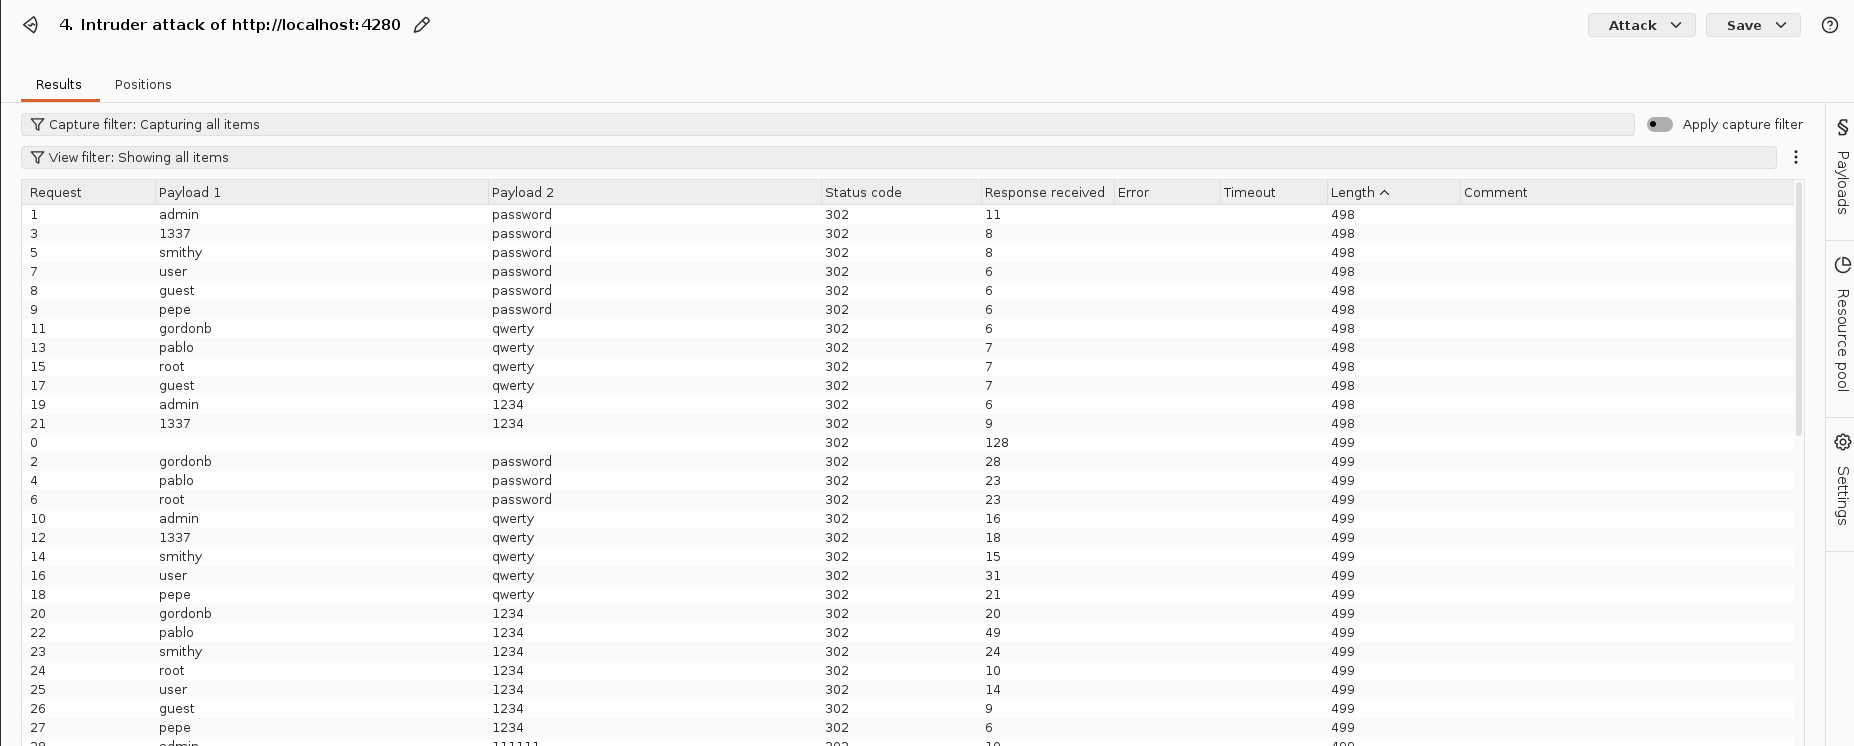
\includegraphics[width=0.95\textwidth]{ataqueburpsuit.png}
    \caption{Ejecución del ataque \textbf{Cluster bomb} en Intruder \textbf{sin sesión válida}: todas las peticiones responden \texttt{HTTP 302} (redirección a \texttt{login.php}). Con una sesión autenticada (Figura~\ref{fig:burp-valido}) pasan a \texttt{200} y el \texttt{Length} delata los aciertos.}
    \label{fig:burp-302}
\end{figure}

\begin{figure}[H]
    \centering
    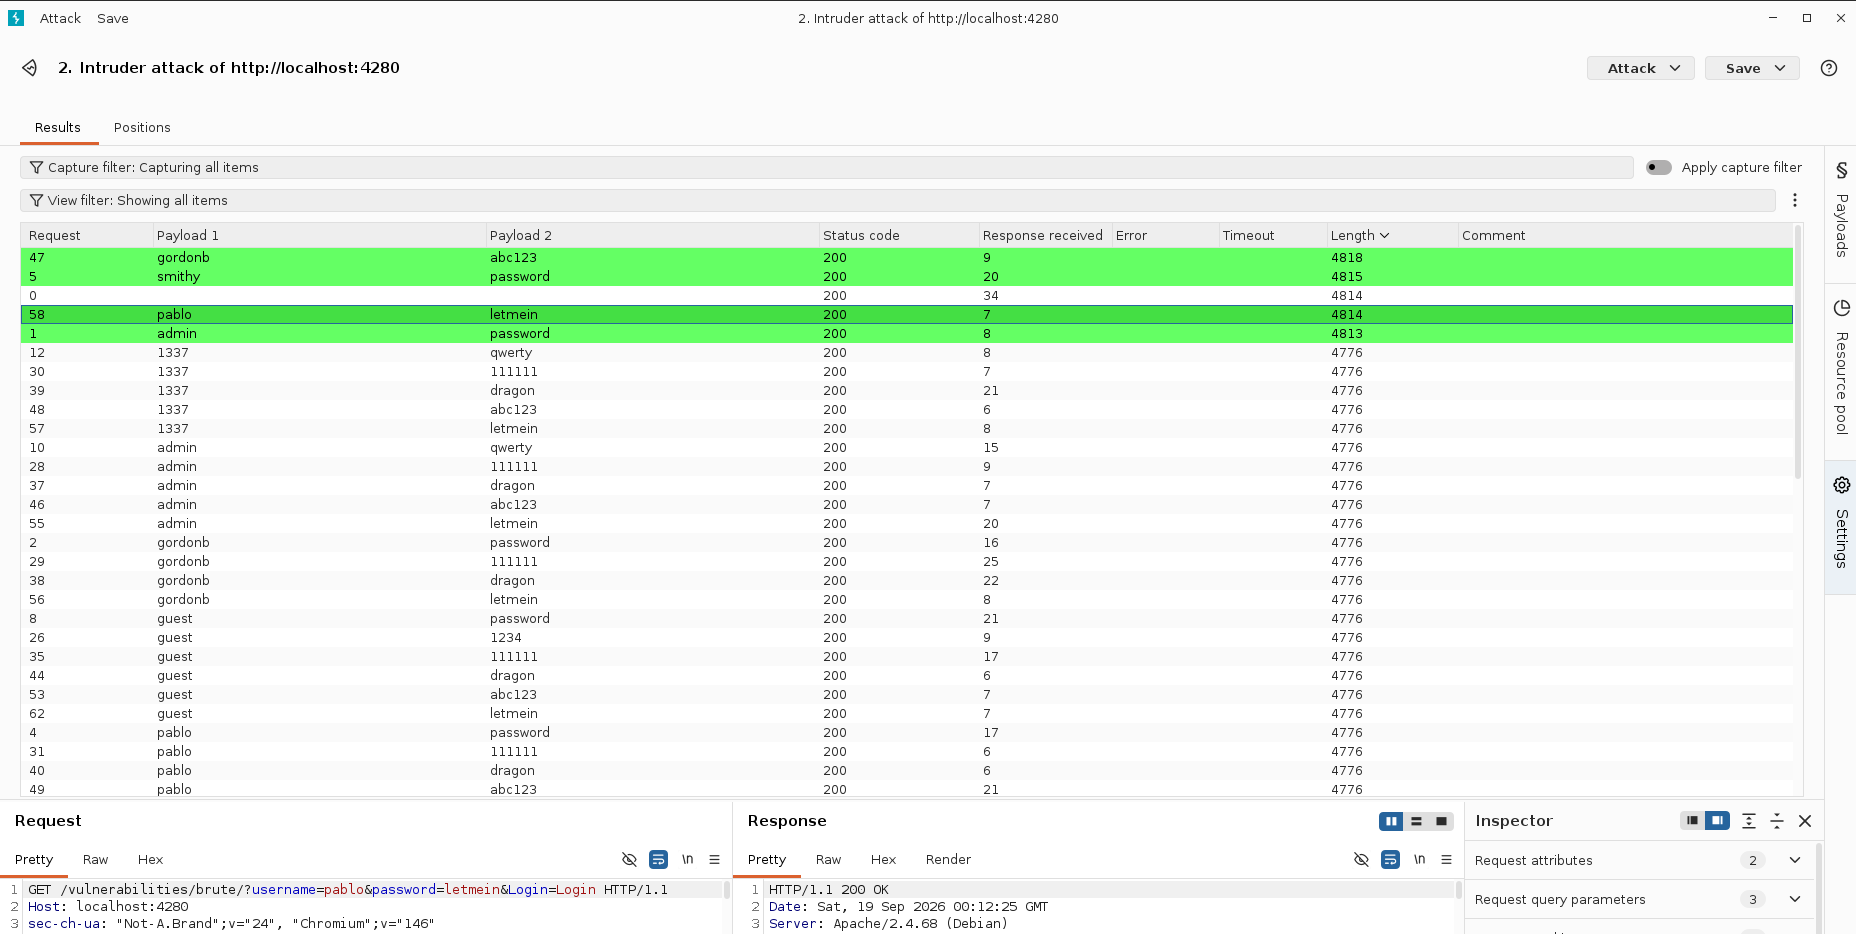
\includegraphics[width=0.95\textwidth]{realcapturaluegodeserunloginreal.png}
    \caption{Resultados con una sesión válida: ordenados por \texttt{Length}, las filas resaltadas (longitud distinta a la baseline) son los logins correctos.}
    \label{fig:burp-valido}
\end{figure}


\textbf{Limitaciones observadas de Burp Suite Community.}

\begin{enumerate}
    \item \textbf{Consumo de memoria:} Intruder carga la wordlist \textbf{completa en RAM}; con diccionarios grandes (\texttt{rockyou}) la herramienta se vuelve inutilizable, por lo que hubo que usar una lista reducida.
    \item \textbf{Throttling deliberado:} la edición Community \textbf{limita la velocidad} de Intruder y no permite ajustar la concurrencia (\emph{Resource pool}), por lo que no sirve para fuerza bruta a escala real.
    \item \textbf{Requiere sesión autenticada previa:} el formulario exige una sesión válida (\texttt{PHPSESSID}); sin un login correcto previo, cada request se \textbf{redirige a \texttt{login.php} (HTTP 302)} y el \emph{Cluster bomb} no prueba nada. Sólo tras obtener un \texttt{200} (sesión válida) el ataque combinatorio funciona.
\end{enumerate}

Estas tres limitaciones justifican por qué, para un ataque de fuerza bruta a escala, se prefieren herramientas como \textbf{Hydra} (multihilo, hace \emph{streaming} del diccionario sin agotar RAM) y por qué \textbf{cURL} se usa para el análisis puntual de una respuesta válida vs. inválida. \\


\subsection{Obtención de código de inspect element (curl)}
Estando autenticado en DVWA (nivel Low), se abrieron las herramientas de desarrollador del navegador (\emph{Inspect Element} $\rightarrow$ pestaña \textbf{Network}) y se envió el formulario de \texttt{Brute Force}. Un solo envío genera decenas de peticiones (el documento HTML más todos sus recursos: CSS, JS, imágenes, avatares, \emph{favicon}); la relevante es el \textbf{documento} cuya URL contiene los parámetros del login. Filtrando por \texttt{brute} (o por tipo \emph{Doc}) se aísla esa petición y, con clic derecho $\rightarrow$ \textbf{Copy $\rightarrow$ Copy as cURL}, se obtiene el comando exacto capturado por el navegador, que queda guardado en \texttt{inspect\_del\_code.txt}. Dicha captura, con la petición del formulario en la pestaña \textbf{Network}, se muestra en la Figura~\ref{fig:curlcode}. \\


De todo lo copiado, lo \textbf{imprescindible} para replicar la petición es: la \textbf{URL con los parámetros} \texttt{username}, \texttt{password} y \texttt{Login}, y la \textbf{cookie} \texttt{PHPSESSID} (de la sesión autenticada) junto con \texttt{security=low}. El resto de cabeceras (\texttt{sec-ch-ua}, \texttt{User-Agent}, etc.) no altera el resultado y puede omitirse. \\


\begin{figure}[H]
    \centering
    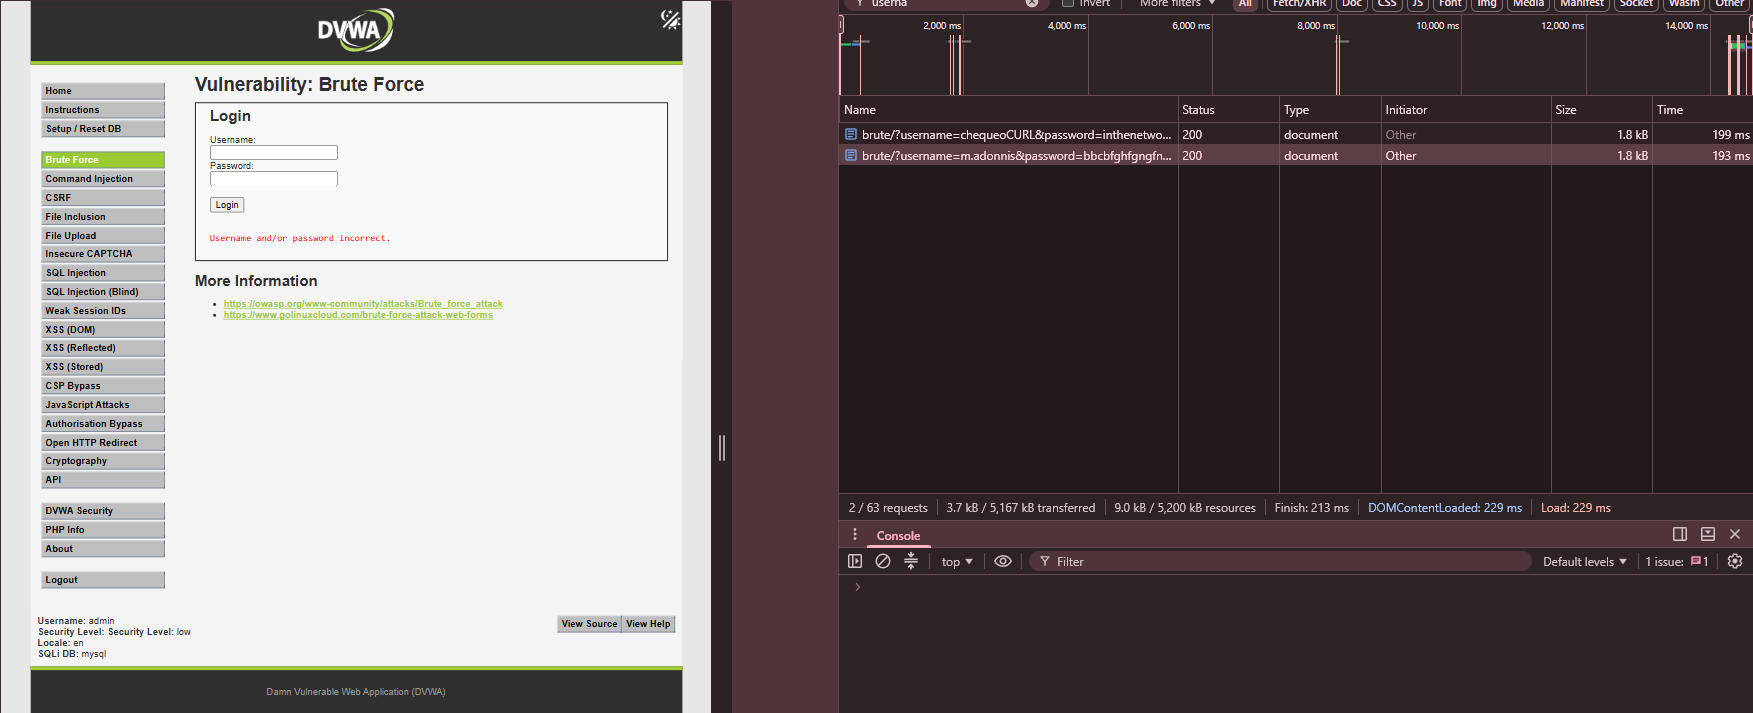
\includegraphics[width=0.95\textwidth]{curl.png}
    \caption{Obtención del código desde \emph{Inspect Element}: la pestaña \textbf{Network} muestra la petición del formulario \texttt{brute} (Status 200, tipo \emph{document}) de la que se copió el comando cURL.}
    \label{fig:curlcode}
\end{figure}

\subsection{Utilización de curl por terminal (curl)}
A partir de esa petición se construyeron dos invocaciones idénticas salvo por las credenciales: un \textbf{acceso válido} con un par real obtenido en el paso de Burp (\texttt{pablo/letmein}) y un \textbf{acceso inválido} con un usuario inexistente (\texttt{m.adonnis}). Ambos comandos quedaron guardados como scripts en \href{https://github.com/maxxee1/crypto-network-security-coursework/tree/main/Lab2/code}{\texttt{Lab2/code/}} (\texttt{curl\_valido.sh}, \texttt{curl\_invalido.sh} y \texttt{curl\_diferencias.sh}): cada invocación envía la cookie de sesión autenticada con \texttt{-b}, guarda el cuerpo HTML con \texttt{-o} y las cabeceras con \texttt{-D}, e imprime con \texttt{-w} un resumen de código HTTP, tamaño y tiempo. La salida obtenida fue: \\


\begin{verbatim}
VALIDO   -> HTTP 200 | 4547 bytes | 0.321s
INVALIDO -> HTTP 200 | 4509 bytes | 0.250s
\end{verbatim}

\newpage
\subsection{Demuestra 5 diferencias (curl)}
Comparando ambas respuestas con \texttt{curl\_diferencias.sh} (que ejecuta \texttt{diff} y \texttt{grep} sobre \texttt{valido.html} e \texttt{invalido.html})\footnote{El script de comparación, las dos respuestas guardadas (\texttt{valido.html}, \texttt{invalido.html}) y sus cabeceras (\texttt{head\_valido.txt}, \texttt{head\_invalido.txt}) están disponibles en el repositorio: \url{https://github.com/maxxee1/crypto-network-security-coursework/tree/main/Lab2/code}.}, la única línea del cuerpo que cambia es:


\begin{verbatim}
80c80
< <p>Welcome to the password protected area pablo</p>
  <img src="/hackable/users/pablo.jpg" />
---
> <pre><br />Username and/or password incorrect.</pre>
\end{verbatim}

De ahí se desprenden las siguientes diferencias entre el acceso válido y el inválido:

\begin{enumerate}
    \item \textbf{Mensaje de resultado:} el válido muestra \emph{``Welcome to the password protected area''}; el inválido, \emph{``Username and/or password incorrect.''}.
    \item \textbf{Imagen de avatar:} el válido incluye \texttt{<img src="/hackable/users/pablo.jpg">}; el inválido no incluye imagen de usuario.
    \item \textbf{Eco del nombre de usuario:} el válido devuelve el \emph{username} autenticado (\texttt{pablo}) dentro del mensaje; el inválido no lo menciona.
    \item \textbf{Estructura HTML:} el válido usa \texttt{<p>...</p>} seguido de \texttt{<img>}; el inválido usa \texttt{<pre><br />...</pre>}.
    \item \textbf{Tamaño de la respuesta / Content-Length:} \textbf{4547} bytes (válido) frente a \textbf{4509} bytes (inválido).
\end{enumerate}

\begin{figure}[H]
    \centering
    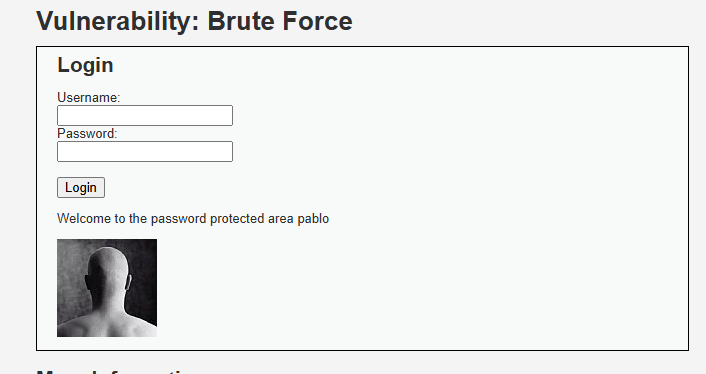
\includegraphics[width=0.6\textwidth]{validacionmanualdelburpsuit.png}
    \caption{Acceso válido (\texttt{pablo/letmein}): la respuesta muestra \emph{``Welcome to the password protected area pablo''} y el avatar del usuario, a diferencia del mensaje de error del acceso inválido.}
\end{figure}

\subsection{Instalación y versión a utilizar (hydra)}
Hydra viene preinstalado en Kali Linux. Se verificó su ruta (\texttt{/usr/bin/hydra}) y su versión, como se muestra en la Figura~\ref{fig:hydra}. La versión utilizada fue \textbf{Hydra v9.7} (van Hauser / THC \& David Maciejak, 2023). De no estar disponible, se instala con \texttt{sudo apt-get install -y hydra}. \\


\begin{figure}[H]
    \centering
    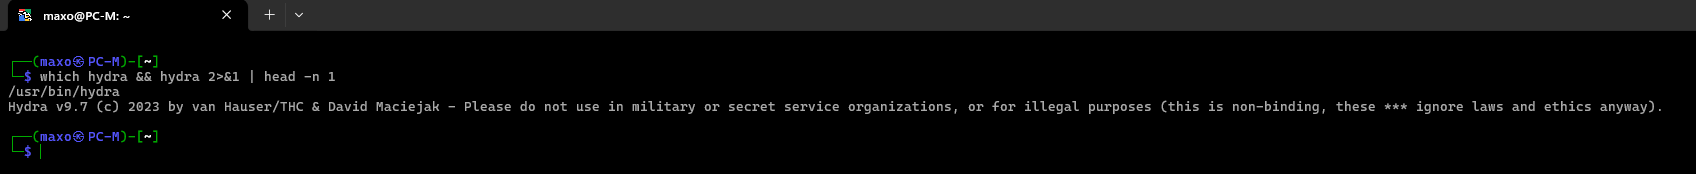
\includegraphics[width=\textwidth]{hydrapreinstalado.png}
    \caption{Verificación de que Hydra está preinstalado (\texttt{/usr/bin/hydra}) y de su versión: \textbf{Hydra v9.7}.}
    \label{fig:hydra}
\end{figure}

\subsection{Explicación de comando a utilizar (hydra)}
Para replicar el formulario de \texttt{Brute Force} (que en nivel Low envía por método GET) se utilizó el módulo \texttt{http-get-form}:

{\footnotesize
\begin{verbatim}
hydra -L users_mod.txt -P 500-worst-passwords.txt 127.0.0.1 -s 4280 http-get-form \
"/vulnerabilities/brute/:username=^USER^&password=^PASS^&Login=Login:H=Cookie\: PHPSESSID=<SID>; security=low:F=Username and/or password incorrect" -V
\end{verbatim}
}

Desglose de cada parte:
\begin{itemize}
    \item \texttt{-L users\_mod.txt}: archivo con la \textbf{lista de usuarios} (\texttt{L} mayúscula = archivo; \texttt{-l} sería un solo usuario). Se usó \texttt{top-usernames-shortlist.txt} de SecLists \textbf{enriquecida} con los usuarios enumerados de DVWA (\texttt{admin}, \texttt{gordonb}, \texttt{1337}, \texttt{pablo}, \texttt{smithy}).
    \item \texttt{-P 500-worst-passwords.txt}: archivo con la \textbf{lista de contraseñas} (\texttt{P} mayúscula), utilizado \textbf{sin modificar} (lista original de SecLists).
    \item \texttt{127.0.0.1 -s 4280}: host y puerto del objetivo.
    \item \texttt{http-get-form}: módulo para formularios enviados por GET. Su cadena tiene \textbf{3 campos separados por} \texttt{:}
    \begin{enumerate}
        \item \texttt{/vulnerabilities/brute/}: ruta del formulario.
        \item Los parámetros del login, donde los marcadores \texttt{\textasciicircum USER\textasciicircum} y \texttt{\textasciicircum PASS\textasciicircum} son sustituidos por Hydra en cada intento con cada usuario y contraseña de las listas.
        \item Condiciones: \texttt{H=Cookie\textbackslash: ...} envía la \textbf{cookie de sesión autenticada} (el \texttt{\textbackslash:} escapa los dos puntos para que Hydra no los tome como separador de campo), y \texttt{F=Username and/or password incorrect} es el \textbf{patrón de fallo}: si la respuesta contiene ese texto el intento es inválido; si no aparece, es un acierto.
    \end{enumerate}
    \item \texttt{-V}: modo verboso (muestra cada intento en pantalla).
\end{itemize}

\subsection{Obtención de al menos 2 pares (hydra)}
Al ejecutar el ataque, Hydra recorrió todas las combinaciones e informó los pares válidos. La corrida finalizó con:
\begin{verbatim}
1 of 1 target successfully completed, 4 valid passwords found
Hydra (https://github.com/vanhauser-thc/thc-hydra) finished at 2026-09-19
\end{verbatim}
Se obtuvieron \textbf{4 pares} usuario/contraseña válidos (muy por encima de los 2 exigidos por la rúbrica):

\begin{table}[H]
\centering
\begin{tabular}{ll}
\hline
\textbf{Usuario} & \textbf{Contraseña} \\
\hline
admin   & password \\
gordonb & abc123 \\
pablo   & letmein \\
smithy  & password \\
\hline
\end{tabular}
\caption{Pares válidos encontrados por Hydra (\texttt{top-usernames-shortlist} enriquecida $\times$ \texttt{500-worst-passwords}).}
\end{table}

El par \texttt{1337/charley} no aparece porque \texttt{charley} no está en \texttt{500-worst-passwords} (es un nombre, no una contraseña común); para recuperarlo bastaría con añadirlo a la lista de contraseñas. Como ventaja frente a Burp Community, se destaca que Hydra procesó la totalidad de las combinaciones \textbf{sin problemas de memoria ni \emph{throttling}}, gracias a su ejecución multihilo y al procesamiento de las listas en \emph{streaming}. \\


\begin{figure}[H]
    \centering
    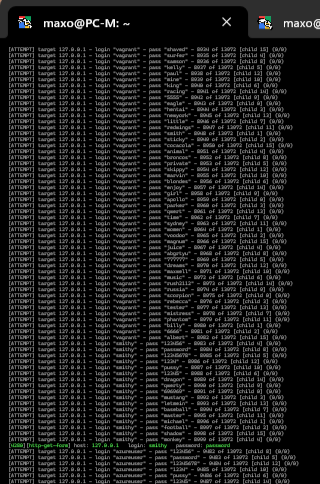
\includegraphics[width=0.5\textwidth]{hydrafounds.png}
    \caption{Salida verbosa de Hydra (\texttt{-V}): las líneas \texttt{[ATTEMPT]} muestran cada combinación probada y las líneas \texttt{[4280][http-get-form]} resaltan los pares válidos encontrados.}
\end{figure}

\subsection{Explicación paquete curl (tráfico)}
El tráfico se capturó en la interfaz \emph{loopback} con \texttt{tcpdump} (\texttt{sudo tcpdump -i lo -s0 -w lab2\_traffic.pcap 'tcp port 4280'}) mientras se lanzaba cada herramienta, y luego se leyó con \texttt{tcpdump -A -r}.

%\begin{figure}[H]
%\centering
%\begin{tikzpicture}[
 % font=\small,
  %tool/.style={draw, rounded corners, thick, align=center, minimum width=3.4cm, minimum height=1cm},
  %server/.style={draw, rounded corners, thick, align=center, fill=gray!12, minimum width=3cm, minimum height=1.5cm}
%]
 % \node[tool, fill=blue!10]  (curl)  at (0,2)  {\textbf{cURL}\\[2pt]\texttt{curl/8.20.0}};
 % \node[tool, fill=red!12]   (hydra) at (0,0)  {\textbf{Hydra}\\[2pt]\texttt{Mozilla/5.0 (Hydra)}};
  %\node[tool, fill=green!16] (burp)  at (0,-2) {\textbf{Burp} (navegador)\\[2pt]\texttt{...Chrome/146...}};
  %\node[server] (dvwa) at (8.2,0) {\textbf{DVWA}\\[2pt]Apache\\[2pt]\texttt{127.0.0.1:4280}};

  %\draw[-{Latex}, thick] (curl.east)  -- (dvwa.west);
  %\draw[-{Latex}, thick] (hydra.east) -- (dvwa.west);
  %\draw[-{Latex}, thick] (burp.east)  -- (dvwa.west);

  %\node[draw, dashed, rounded corners, inner sep=13pt,
   %     fit=(curl)(hydra)(burp)(dvwa),
    %    label={[align=center]above:{\textbf{Interfaz \texttt{lo} (loopback)}\\[-1pt]\texttt{sudo tcpdump -i lo 'tcp port 4280'}}}] {};
%\end{tikzpicture}
%\caption{Topología de la captura: las tres herramientas atacan a DVWA sobre la interfaz \emph{loopback}, donde \texttt{tcpdump} registra todo el tráfico HTTP en claro.}
%\label{fig:topo}
%\end{figure}

\begin{figure}[H]
    \centering
    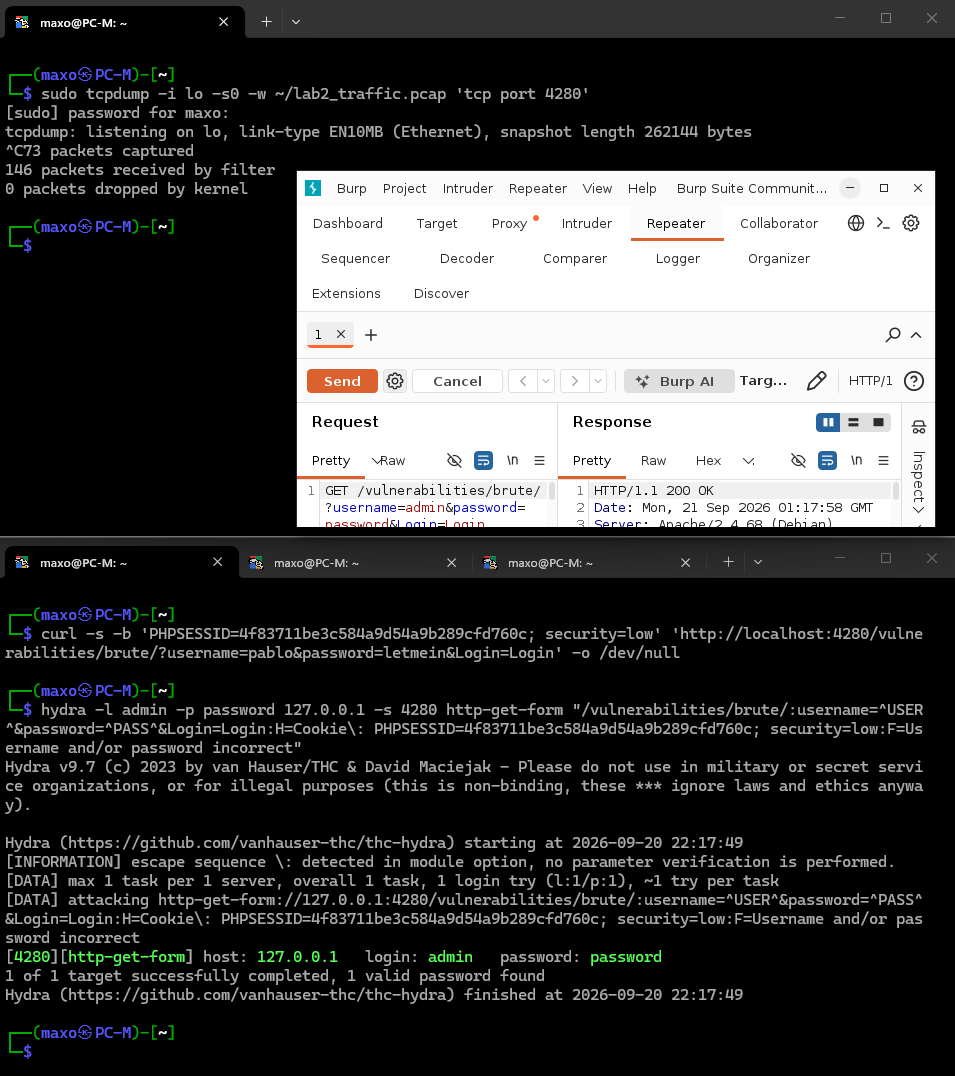
\includegraphics[width=0.85\textwidth]{2terminales_leyendotraficohydra_curl_burp.png}
    \caption{Montaje de la captura: \texttt{tcpdump} grabando en \texttt{lo} (arriba a la izquierda), Burp enviando una petición desde Repeater, y las corridas de cURL y Hydra contra \texttt{127.0.0.1:4280}.}
\end{figure}
\newpage

La petición generada por cURL fue:

\begin{verbatim}
GET /vulnerabilities/brute/?username=pablo&password=letmein&Login=Login HTTP/1.1
Host: localhost:4280
User-Agent: curl/8.20.0
Accept: */*
Cookie: PHPSESSID=4f83711be3c584a9d54a9b289cfd760c; security=low
\end{verbatim}

Es una petición \textbf{mínima}: \texttt{HTTP/1.1} con solo 4 cabeceras (\texttt{Host}, \texttt{User-Agent}, \texttt{Accept} y \texttt{Cookie}). El \texttt{User-Agent} es literalmente \texttt{curl/8.20.0} y el \texttt{Accept} es el genérico \texttt{*/*}. No incluye ninguna cabecera propia de un navegador.

\subsection{Explicación paquete burp (tráfico)}
La petición reenviada por Burp al servidor fue:

{\footnotesize
\begin{verbatim}
GET /vulnerabilities/brute/?username=...&password=...&Login=Login HTTP/1.1
Host: localhost:4280
sec-ch-ua: "Not-A.Brand";v="24", "Chromium";v="146"
sec-ch-ua-mobile: ?0
sec-ch-ua-platform: "Linux"
Accept-Language: en-US,en;q=0.9
User-Agent: Mozilla/5.0 (X11; Linux x86_64) AppleWebKit/537.36 (KHTML, like
            Gecko) Chrome/146.0.0.0 Safari/537.36
Accept: text/html,application/xhtml+xml,application/xml;q=0.9,image/avif,...
Sec-Fetch-Site: same-origin
Sec-Fetch-Mode: navigate
Sec-Fetch-User: ?1
Sec-Fetch-Dest: document
Referer: http://localhost:4280/vulnerabilities/brute/?username=...
Cookie: PHPSESSID=00b8aabbe116e3660668bc59f8390bf6; security=low
Connection: keep-alive
Connection: Keep-Alive
\end{verbatim}
}

A diferencia de cURL, Burp envía el \textbf{conjunto completo de cabeceras de un navegador} porque \textbf{reenvía la petición original} de su navegador embebido: \texttt{User-Agent} de Chrome, \texttt{sec-ch-ua*}, \texttt{Sec-Fetch-*}, \texttt{Accept-Language}, \texttt{Referer} y un \texttt{Accept} de tipo \texttt{text/html,\ldots}. Un detalle revelador es la cabecera \texttt{Connection} \textbf{duplicada} (\texttt{keep-alive} del navegador y \texttt{Keep-Alive} que añade el proxy), artefacto típico de Burp. \\


\subsection{Explicación paquete hydra (tráfico)}
La petición generada por Hydra fue:

\begin{verbatim}
GET /vulnerabilities/brute/?username=admin&password=password&Login=Login HTTP/1.0
Cookie:  PHPSESSID=4f83711be3c584a9d54a9b289cfd760c; security=low
Host: 127.0.0.1:4280
User-Agent: Mozilla/5.0 (Hydra)
Connection: close
\end{verbatim}

Hydra también manda pocas cabeceras, pero con varias huellas distintivas: usa \textbf{HTTP/1.0} (versión más antigua), su \texttt{User-Agent} es \texttt{Mozilla/5.0 (Hydra)} (firma delatandose), añade \texttt{Connection: close}, coloca la cabecera \texttt{Cookie} \textbf{antes} de \texttt{Host} (orden atípico) con un doble espacio (\texttt{Cookie:\ \ PHPSESSID}), usa la IP en \texttt{Host} y \textbf{omite} el \texttt{Accept}. Además, antes del intento de login realiza una petición \emph{previa} a \texttt{/vulnerabilities/brute/} (sin parámetros) para cargar el formulario. \\


\subsection{Mención de las diferencias (tráfico)}
Comparando los tres paquetes:

\begin{table}[H]
\centering
\renewcommand{\arraystretch}{1.25}
\begin{tabular}{l >{\columncolor{blue!8}}l >{\columncolor{red!8}}l >{\columncolor{green!10}}l}
\rowcolor{gray!30}
\textbf{Aspecto} & \textbf{cURL} & \textbf{Hydra} & \textbf{Burp} \\
\hline
Versión HTTP          & 1.1           & \textbf{1.0}                 & 1.1 \\
User-Agent            & \texttt{curl/8.20.0} & \texttt{Mozilla/5.0 (Hydra)} & Chrome (navegador) \\
Nº de cabeceras       & 4 (mínimas)   & 5 (mínimas)                  & $\sim$14 (completas) \\
Accept                & \texttt{*/*}  & (ausente)                    & \texttt{text/html,\ldots} \\
Connection            & (por defecto) & \texttt{close}               & \textbf{keep-alive duplicada} \\
sec-ch-ua / Sec-Fetch & no            & no                           & sí \\
Orden de cabeceras    & Host primero  & \textbf{Cookie primero}      & Host primero \\
\hline
\end{tabular}
\caption{Diferencias entre los paquetes generados por cada herramienta (columnas coloreadas por herramienta; en negrita las huellas más delatoras).}
\end{table}

En síntesis: cURL y Hydra producen peticiones \textbf{escuetas y de aspecto automatizado} (pocas cabeceras, \texttt{Accept} genérico o ausente), mientras que Burp produce una petición \textbf{indistinguible de un navegador} porque reenvía la original. Hydra se diferencia además por usar HTTP/1.0 y un orden de cabeceras poco natural. \\


\begin{figure}[H]
    \centering
    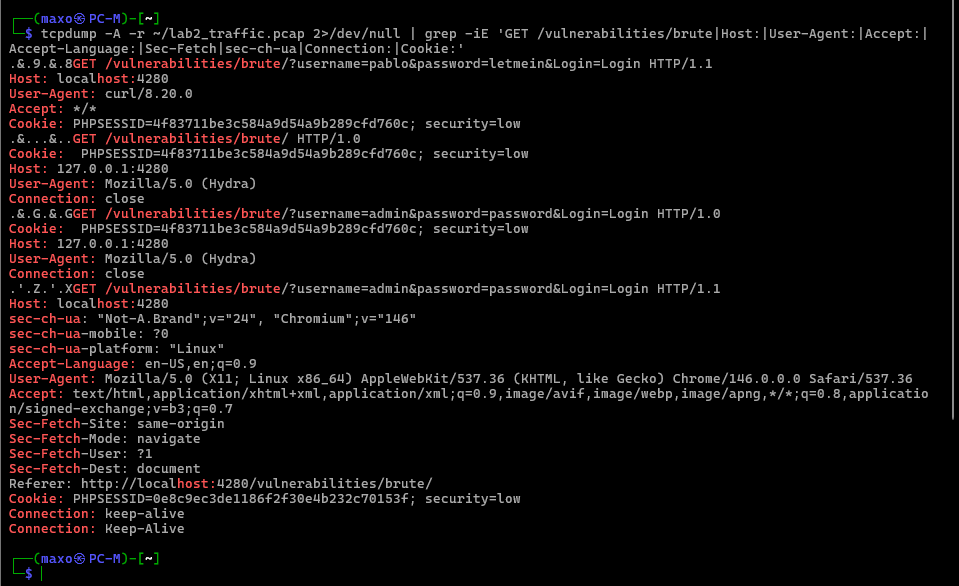
\includegraphics[width=0.95\textwidth]{cabecerascompletas_cadapeticion.png}
    \caption{Cabeceras completas de las tres peticiones (cURL, Hydra y Burp) leídas del \texttt{.pcap} con \texttt{tcpdump -A}: se aprecian las diferencias en versión HTTP, \texttt{User-Agent}, y orden y cantidad de cabeceras.}
\end{figure}

\subsection{Detección de SW (tráfico)}
Sí es posible identificar la herramienta que originó cada paquete:
\begin{itemize}
    \item \textbf{cURL:} trivial. El campo \texttt{User-Agent: curl/8.20.0} lo delata directamente.
    \item \textbf{Hydra:} igualmente trivial. Su \texttt{User-Agent: Mozilla/5.0 (Hydra)} contiene literalmente el nombre de la herramienta; a ello se suman el uso de \textbf{HTTP/1.0}, el \texttt{Connection: close}, el orden \texttt{Cookie} antes de \texttt{Host} y la ausencia de \texttt{Accept}.
    \item \textbf{Burp:} es el \textbf{más difícil} de detectar porque reenvía la petición real del navegador (mismo \texttt{User-Agent} de Chrome y todas sus cabeceras). Aun así deja rastros: la cabecera \texttt{Connection} \textbf{duplicada} (\texttt{keep-alive} + \texttt{Keep-Alive}) es un artefacto del proxy, y a nivel de comportamiento un ataque con Intruder genera una \textbf{ráfaga de peticiones idénticas y muy seguidas}, patrón poco habitual en un usuario real.
\end{itemize}
En conclusión, las herramientas automáticas (cURL y Hydra) se identifican de inmediato por su \texttt{User-Agent}; Burp exige un análisis más fino (anomalías de cabeceras y patrón temporal de las peticiones), pero también resulta detectable. \\ 

\begin{figure}[H]
    \centering
    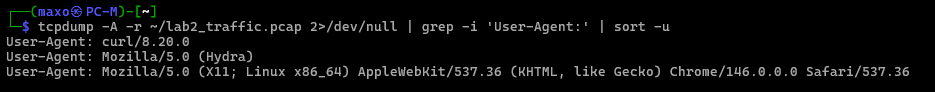
\includegraphics[width=\textwidth]{3traficos_firmas.png}
    \caption{Las tres firmas \texttt{User-Agent} extraídas del \texttt{.pcap}: \texttt{curl/8.20.0}, \texttt{Mozilla/5.0 (Hydra)} y el \texttt{User-Agent} de Chrome (Burp). Los dos primeros delatan la herramienta directamente.}
\end{figure}


% Please add the following required packages to your document preamble:
%\begin{table}[htbp]

\section*{Conclusiones y comentarios}
\addcontentsline{toc}{section}{Conclusiones y comentarios}

El laboratorio permitió ejecutar y comparar un ciclo completo de ataque de fuerza bruta contra el formulario \texttt{vulnerabilities/brute} de DVWA, empleando tres herramientas con propósitos distintos. La principal conclusión es que \textbf{no existe una única herramienta ``mejor''}: cada una cumple un rol diferenciado.

\begin{itemize}
    \item \textbf{Burp Suite (Community):} excelente para \emph{interceptar, entender y modificar} la petición (Intruder, \emph{Positions}, Cluster bomb), pero \textbf{inadecuada para fuerza bruta a escala}. Carga el diccionario completo en RAM, ya que \texttt{rockyou} la volvió inutilizable, y la edición gratuita \emph{throttlea} deliberadamente el ataque, además exige una sesión autenticada previa (\texttt{PHPSESSID}), sin la cual todo se redirige a \texttt{login.php}. Sirve como prueba de concepto controlada, no como motor de ataque masivo.
    \item \textbf{Hydra:} la herramienta \emph{correcta para la escala}. Multihilo y procesando las listas en \emph{streaming}, resolvió más de $10^{4}$ combinaciones sin problemas de memoria ni de velocidad. Su desventaja es que es \textbf{ruidosa}: su \texttt{User-Agent} (\texttt{Mozilla/5.0 (Hydra)}) y el uso de HTTP/1.0 la delatan de inmediato.
    \item \textbf{cURL:} herramienta \emph{de precisión}. No apunta al volumen, sino a \textbf{replicar una petición puntual} y comparar con precisión un acceso válido frente a uno inválido (5 diferencias observadas). Ideal para el análisis fino.
\end{itemize}

Desde el punto de vista de la \textbf{seguridad de la aplicación}, se evidenciaron varias debilidades encadenadas en el nivel Low:
\begin{itemize}
    \item \textbf{Credenciales débiles:} todas las contraseñas por defecto se recuperaron con listas públicas comunes, y los hashes se almacenan como \textbf{MD5 sin sal}, crackeables en segundos.
    \item \textbf{Exposición por método GET:} usuario y contraseña viajan \textbf{en la propia URL}, quedando expuestos en el historial del navegador, los \emph{logs} del servidor y la cabecera \texttt{Referer}.
    \item \textbf{Ausencia de mitigaciones:} en Low no hay bloqueo ni límite de intentos.
    
    \item \textbf{Fuga de información:} los nombres de usuario no son secretos y se enumeraron mediante \textbf{SQL Injection} (volcado de la tabla \texttt{users}), reduciendo el espacio de búsqueda del atacante.
\end{itemize}

El análisis de \textbf{tráfico} mostró que cada herramienta deja una \textbf{huella identificable}: cURL y Hydra se detectan trivialmente por su \texttt{User-Agent}, mientras que Burp es más sigiloso al reenviar la petición real del navegador, aunque delatable por artefactos del proxy (cabecera \texttt{Connection} duplicada) y por el patrón de ráfaga de Intruder. La lectura \textbf{defensiva} es directa: un IDS/WAF puede bloquear firmas de herramientas automáticas, por lo que un atacante que busque sigilo recurrirá a proxies que imiten al navegador. \\


Como comentario final, operar una aplicación \emph{deliberadamente vulnerable} exigió \textbf{aislar el entorno} (publicación solo en \texttt{loopback}, red \emph{bridge} dedicada, contenedores sin privilegios y desmontaje de \texttt{/mnt/c}). En conjunto, el laboratorio no solo ejercita la técnica ofensiva, sino que hace evidentes las defensas que la neutralizan: \textbf{contraseñas robustas con hash salado, envío por POST sobre HTTPS, límites de intentos y bloqueo de cuentas, mensajes de error genéricos y monitorización de firmas de herramientas}. \\


\end{document}